\documentclass[12pt, letterpaper, oneside]{article}
\usepackage[utf8]{inputenc}
\usepackage[LGR,T1]{fontenc}
\usepackage{braket}
\usepackage{amsmath}
\usepackage{biblatex}
\usepackage{bbold}
\usepackage{quantikz}

\addbibresource{refx.bib}
\newtheorem{definition}{Definicija}
\renewcommand{\figurename}{Slika}

\title{Kvantno mašinsko učenje}
\author{Milan Bojić}
\date{Septembar 2022.}

\renewcommand*\contentsname{Sadržaj}

\begin{document}

\maketitle
\newpage

\tableofcontents
\newpage
\section{Uvod}
Prethodna decenija je bila obeležena mašinskim učenjem, sa njegovom primenom u svakodnevnom životu običnih ljudi.
Međutim, u prethodnih nekoliko godina počelo je da se oseća usporenje inovacija i razvoja novih metoda, a u nekim oblastima su i dostignute granice računarskih resursa (npr. GPT-3).
U rešavanju ovog problema očekuje se da pomogne razvoj kvantnog računarstva, oblasti koja  se razvija gotovo pola veka, ali tek u poslednjih nekoliko godina je došlo do
povećanog interesovanja. Za kvantno računarstvo se očekuje da bude sledeće veliko remećenje tehnološkog poretka, sa približavanjem kvantnoj nadmoći svakog dana.

Od kvantnog mašinskog učenja se očekuje da bude prekretnica u mašinskom učenju kakvo danas znamo. Oblast je relativno mlada i trenutno se najviše bavi teoretskim razvojem.
Neki od zadataka kojim se bavi jeste obrada kvantnih sistema i ``učenje'' njihovih osobina, brže i bolje prepoznavanje obrazaca u klasičnom sistemu, kao i
otkrivanje nekih osobina klasičnog mašinskog učenja koje se nisu mogle primetiti u klasičnom sistemu.

U ovom radu će biti uvedene u osnove kvantnog računarstva i predstavljeno nekoliko metoda kvantnog mašinskog učenja koji su bili istraživani u prethodnom periodu.

\newpage
\section{Kvantno računarstvo}
Pre nego što se počne pričati o Kvantnom mašinskom učenju, treba objasniti neke osnovne pojmove da bi se ostatk rada mogao lakše razumeti.

\subsection{Osnovni pojmovi}
Potrebni pojmovi su:
\begin{itemize}
    \item Kubit (engl. Qubit)
    \item Kvantna kapija (engl. Quantum Gates)
    \item Kvantna spletenost (engl. Quantum entanglement)
    \item Kvantna memorija, Kvantni registri
\end{itemize}

\subsubsection*{Kubit}
Kubit (engl. Qubit) je najmanja jedinica informacije u kvantnom računarstvu, slično bit-u u klasičnom računarstvu.
Razlika od bita jeste u tome što kubit pored stanja 1 i 0, može da se nalazi i u superpoziciji između oba.
Oni se mogu predstaviti formulom (koristeći bra-ket notaciju):
\[ \ket{\gamma} =  \alpha\ket{0}+\beta\ket{1} \]
Ovde su $\ket{0}$ i $\ket{1}$ zapravo stanja kao i kod klasičnog bita, a $\alpha$ i $\beta$ su kompleksni brojevi koji predstavljaju amplitude zadatih stanja i za njih važi:

\[ |\alpha|^2+|\beta|^2 = 1 \]
Stanje kubita ima dva stepena slobode što dovodi do toga da amplitude se mogu zapisati kao:
\[
    \alpha = \cos{\frac{\Theta}{2}} 
\]
\[
    \beta = e^{i\phi}\sin{\frac{\Theta}{2}}
\]
gde je $e^{i\phi}$ relativna faza kubita, a $\Theta$ ugao.

Jedna od mogućih načina vizualizacije kvantnog stanja kubita jeste pomoću \textbf{Blohove sfere} (Slika 1).
Vizualizovano na sferi, klasični biti su na ``polovima'' sfere, na lokacijama gde se $\Ket{0}$ i $\Ket{1}$  takođe nalaze.
Ostatak površine sfere je nepristupačan za klasičan bit, ali stanje kubita može se predstaviti bilo kojom tačkom na površini.
Površina Blohove sfere je dvodimenzionalna, zato stanje kubita ima dva stepena slobode i može se predstaviti preko uglova $\phi$ i $\Theta$.
\begin{figure*}[ht]
    \centering
    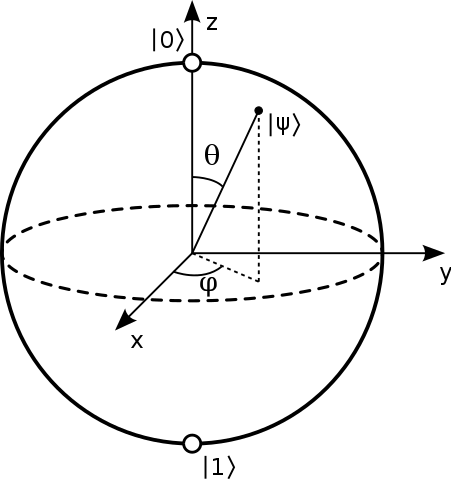
\includegraphics[width=0.5\textwidth]{files/Bloch_sphere.png}
    \caption{Vizuelizacije kvantnog stanja kubita pomoću Blohove sfere\cite{BlochSphereImage}}
\end{figure*}

Takođe možemo da vidimo da je $|\alpha|^2$ verovatnoća da se kubit nalazi u stanju 0, isto važi i za $ |\beta|^2$ i 1.
Saznanje o tome u kom stanju se nalazi kubit se dobija merenjem kubita, kada bi kubit izašao iz superpozicije i ``pao'' u stanje 1 ili stanje 0. U tom slučaju kubit će imati ponašanje kao i običan bit, ali ovako gubimo pređašnje kvantno stanje kubita.
U fizičkom svetu kubit se može predstaviti kao polarizovan foton,gde će dva stanja da se uzimaju kao vertikalna i horizontalna polarizacija.
\subsubsection*{Kvantna kapija}
Kvantne kapije (engl. Quantum Gates) su logički predstavljene matricama i one rade nad određenim brojem kubita.
Matrice su unitarne sa oblikom $2^n \times 2^n$, gde je $n$ broj kubita sa kojim radimo. Neke od poznatih kola su: Hademardovo kolo (stavlja kubit u superpoziciju)
\[
    H = \frac{1}{\sqrt{2}}\begin{bmatrix}
        1 & 1 \\
        1 & -1
    \end{bmatrix}
\]
Pauli-jeva kola (zamenjuju amplitude na kubitu po osama), ali nas najviše zanima rotaciono kolo:
\[
    R = \begin{bmatrix}
        \cos{\Theta} & -\sin{\Theta} \\
        \sin{\Theta} & \cos{\Theta} 
    \end{bmatrix}
\]
Ovo kolo rotira kubite u prostoru, odnosno menja njihove amplitude za $\Theta$ radijana.
%% Pogledati Quantum Computation and Quantum Information chap. 1.3 Quantum computation za dopune
\subsubsection*{Kvantna spletenost}
Kvantna spletenost (engl. Quantum entanglement) je fizički pojam gde su dva, ili više, kubita povezana tako da zajedno prave novo kvantno stanje.
U čistim stanjima oni su matematički zapravo proizvodi tenzora amplituda:
\[
    \ket{\gamma} \otimes \ket{\delta} = \alpha_1\alpha_2\ket{00} + \alpha_1\beta_2\ket{01} + \beta_1\alpha_2\ket{10} + \beta_1\beta_2\ket{11}
\]
I ovako napisano kvantno stanje se može razdvojiti na dva kubita. Ali postoje i kvanta stanja koja se ne mogu razdvojiti npr.
\[
 \frac{1}{\sqrt{2}}\ket{00} + \frac{1}{\sqrt{2}}\ket{11}
\]
Zanimljiva stvar kod spletenih kubita jeste u tome što dele informacije. Ako bi jedan kubit iz para odneli u neko veoma daleko mesto (na primer druga galaksija),
i tamo bi ga izmerili, dobili bi smo 0 ili 1, međutim drugi kubit bi takođe upao u određeno stanje i to u istom trenutku kad smo izmerili prvi daleki kubit.
Ovo je zapravo gde se nalazi glavna različitost između klasičnog i kvantnog računarstva, ova pojava ne postoji u klasičnom računarstvu i ne može se "lako" simulirati.
\subsubsection*{Kvantni registri}
Kvantni registri se sastoje od kvantnog stanja od $m$ spletenih kubita i mogu predstavljati do $2^m$ vrednosti stanja istovremeno.
Kvantna memorija su uređaji koji čuvaju kvantna stanja fotona, bez uništavanja kvantne informacije koja se nalazi u fotonu.
Ovakva memorija zahteva koherentni sistem materijala, jer bi u suprotnom kvantna informacija unutar uređaja bila izgubljena zbog nekoherentnosti.

\subsection{Kvantno računarstvo}
Kvantno računarstvo je vrsta računarstva gde se koriste kolekcije fizičkih osobina kvantne mehanike kao što su superpozicija i kvantna spletenost,
tako da se izvrši neka kalkulacija. Uređaji koji izvršavaju kvantne kalkulacije zovu se \textbf{kvantni računari} (Slika 2).
Kvantni računari se sastoje od kvantnih kola i elementarnih kvantnih kapija koje služe za prenošenje i manipulisanje kvantnih informacija.
\cite{nielsen_chuang_10th} \\
Jedna od glavnih primena kvantnih računara jeste simulacija fizičkih sistema, bili oni kvantne ili klasične prirode.
%% Pogledati Quantum Computation and Quantum Information za dopune
\begin{figure*}[ht]
    \centering
    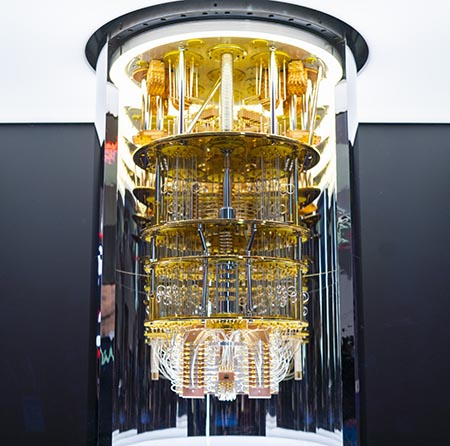
\includegraphics[width=0.5\textwidth]{files/media_sizes_full_QC-stack-fig-2.jpg}
    \caption{Slika spoljašnjosti kvantnog računara \cite{QuantumComputerImage}}
\end{figure*}

\subsection{Kvantna informacija}
Kvantna informacija je informacija o stanju kvantnog sistema. Njihovim svojstvima bavi se \textbf{kvantna teorija informacije}.
Takođe, kvantne informacije se mogu izmeriti na isti način kao i klasična informacija koristeći se \textit{Šenonovom metodom}. 
Postoji jedinstveno merilo, to jest funkcija nad kvantnim stanjem, koja je funkcija verovatnoće, kontinuiteta i sumiranja.\cite{vlatko_v}
Ova funkcija se zove \textbf{fon Nojmanova entropija} i za neki ulazni kubit $\varrho$ postoji ekvivalent u \textbf{Šenonovoj entropiji} $H$
za neku slučajnu promenljivu $X$
\[
    S(\varrho) = H(X)
\]
%% Opisati metod u Appendix-u možda
Još jedno od merila za kvantno stanje jeste merenje validnosti (engl. fidelity) između dva kvantna stanja $\ket{\phi}$ i $\ket{\psi}$.
Neka je $F$ funkcija koja meri osobinu, odnostno meri verovatnoću da merenjem stanja $\ket{\phi}$ dobijemo stanje $\ket{\psi}$.
Izlaz funkcije je između 0 i 1, gde ako je izlaz 0 onda su dva stanja ortogonalna jedna od drugog, a ako je izlaz 1 onda su dva stanja jednaka \cite{vlatko_v}.
\subsubsection*{Odnos kvantne i klasične teorije informacije}
Kvantna i klasična informacija se u dosta stvari razlikuju.  Klasična informacija prolazi kroz sisteme sa dobro definisanim stanjima, može se kopirati i pri procesu merenja se ne menja.
Kvantna informacija je kodirana u kvantnim sistemima, ne može se kopirati i pri procesu merenja ona se menja. Takođe kvantna informacija ima neke osobine koje se ne
mogu iskazati u klasičnoj informaciji, kao što su superpozicija i kvantna spletenost \cite{Classical&quantum_info}. \\
Kvantna teorija informacije se bavi: 
\begin{enumerate}
    \item Prenošenjem klasičnih informacija preko kvantnih kanala
    \item Prenošenjem kvantnih informacija preko kvantnih kanala
    \item Efektima kvantne spletenosti na prenošenje informacija
    \item Informacionm aspektma kvantnog merenja, odnosa između distribucije \\
    kvantnog stanja i preciznog merenja
\end{enumerate}
\subsubsection{Priprema podataka}
Za obradu podataka treba nam kvantni RAM (QRAM), koji nam dozvoljava paralelan pristup kvantnim podacima.
Neka imamo kompleksan vektor $\overrightarrow{v}$ sa $N=2^n$ dimenzija, gde su njegove komponente oblika 
\[
    v_j = |v'_j|e^{i\varphi_j}
\]

Ako imamo parove $\{|v'_j|,\varphi_j\}$, čuvamo ih kao realne brojeve u QRAM-u, onda možemo da konstruišemo
$\log_{2}N$ kvantnih stanja $\ket{v} = |\overrightarrow{v}|^{-\frac{1}{2}}\overrightarrow{v}$ u $O(\log N)$ koraka

Kada smo kreirali kompresovane kvantne vektore od ulaznih vektora, možemo da vršimo transformacije koristeći kvantne algoritme, za dalje korišćenje podataka za mašinsko učenje.
Ovaj proces zove se \textbf{pred procesiranje} i u opštem obliku njemu je potrebno $O(poly(\log{}N))$ koraka \cite{lloyd2013quantum}.

\subsection{Linearna algebra za kvantno mašinsko učenje}
Da bi se videlo kako kvantni računari poboljšavaju mašinsko učenje, treba da se vidi kako kvantni računari obrađuju linearnu algebru, jednu od osnova modernog mašinskog učenja. \\
Tokom godina razvijeno je nekoliko kvantnih algoritama koji rešavaju probleme linearne algebre.
Zajedno ti algoritmi se nazivaju \textbf{osnovni kvantni podprogrami linearne algebre} (engl. qBLAS), i oni se koriste u izradi algoritama za kvantno mašinsko učenje.

Primeri algoritama koji su deo qBLAS-a su: 
\begin{itemize}
    \item HHL algoritam: koristi se za rešavanje sistema linearnih jednačina, koristeći $2^n$-dimenzioni vektorski prostor
        za rešavanje sistema sa $n$ promenljivih \cite{Quantum_machine_learning}.
    \item Kvantna Furijeova transformacija \cite{Classical&quantum_info_Fourie_Phase}.
    \item Kvantna procena faza za sopstvene vrednosti i sopstvene vektore/stanja \cite{Classical&quantum_info_Fourie_Phase}.
\end{itemize}
Ovi algoritmi su korišćeni kao osnova naprednih metoda i algoritama za Kvantno mašinsko učenje.
Samo treba pripaziti kod pominjanja ovih algoritama, jer neki od njih koriste neke koncepte koji su samo teorijske prirode ili su teško kreirani u realnom svetu (npr. QRAM).

\newpage
\section{Kvantna teorija kompleksnosti i kvantni algoritmi}
U klasičnoj teoriji kompleksnosti klasifikuju se algoritamski problemi po njihovoj težini rešavanja.
Problemi se klasifikuju u \textbf{klase kompleksnosti}, koje se mogu posmatrati kao kolekcija algoritamskih problema koji dele neke zajedničke osobine
vezane za računske resurse potrebne da bi se rešili (uglavnom vreme i prostor) \cite{nielsen_chuang_10th}.

\subsection{Primeri klasa kompleksnosti}
Među najpoznatijim i najvažnijim klasama su \textbf{P} i \textbf{NP}. Zbog prirode kvantnih računara biće objašnjene neke druge klase kompleksnosti.

Klasa kompleksnosti \textbf{PSPASE} je klasa problema koji se mogu rešiti u polinomskom prostoru, ali sa neograničenim vremenom izvršavanja.


Klasa kompleksnosti \textbf{PP} (Probabilistic Polynomial-Time) je klasa problema za koje postoji nasumični algoritam u polinomskom vremenu koji vraća
tačno rešenje sa verovatnoćom većom od $\frac{1}{2}$.

Klasa kompleksnosti \textbf{BPP} (Bounded-Error Probabilistic Polynomial-Time) je klasa problema za koje postoji nasumični algoritam u polinomskom vremenu koji vraća
tačno rešenje sa verovatnoćom većom od $\frac{2}{3}$ \cite{aaronson2013quantum}.
\subsection{BQP}
Klasa kompleksnosti \textbf{BQP} (Bounded-Error Quantum Polynomial-Time) je klasa problema koji se mogu efikasno rešiti na kvantnom računaru, ako se dopusti ograničena verovatnoća greške \cite{nielsen_chuang_10th}.
Formalnija definicija bi bila \cite{aaronson2013quantum}:
\begin{definition}
    \textbf{BQP} je klasa jezika $L \subseteq \{0,1\}^{*}$ za koje postoji uniformni skup kvantnih kola polinomske veličine ($C_n$)
    tako da za svako $x \in \{0,1\}^{n}$:
    \begin{itemize}
        \item ako $x \in L$ onda $C_n$ prihvata ulaz $\Ket{x}\Ket{0...0}$ sa verovatnoćom većom od $\frac{2}{3}$.
        \item ako $x \notin L$ onda $C_n$ prihvata ulaz $\Ket{x}\Ket{0...0}$ sa verovatnoćom ne većom od $\frac{1}{3}$.
    \end{itemize} 
\end{definition}
Ovako definisano, može se primetiti da problemi iz \textbf{BQP} su dosta bliži problemima iz \textbf{BPP} nego iz \textbf{P}.
\subsubsection*{Odnos sa klasičnim klasama kompleksnosti}
Prva stvar koja važi jeste da $\textbf{BPP} \subseteq \textbf{BQP}$, odnosno da sve što može da se uradi sa klasičnom probalističkim računarom može da 
se uradi i na kvantnom računaru.

Kada se traži gornja granica kvantnih problema prvo se dolazi do $\textbf{BQP} \subseteq \textbf{EXP}$, ovo znači da kvantni računari mogu da dovedu
do najviše \textit{eksponencijalnog ubrzanja} u odnosu na klasični računar \cite{aaronson2013quantum}.
Bolja gornja granica za $\textbf{BQP}$ jeste $\textbf{BQP} \subseteq \textbf{PP}$. Ovo su dokazali Adleman, DeMarrais i Huang u \cite{adleman1997quantum}.
\subsection{Primeri kvantnih algoritama}
\subsubsection{Šorov algoritam}
Trenutno optimalan algoritam na klasičnom računaru (\textit{general number filed sieve}) se izvršava u sub-eksponencijalnom vremenu.
Šorov algoritam rešava problem nalaženja periode, koji može da se iskoristi za problem faktorizacije \cite{QiskiShoreAlgo}.\\
\textbf{Problem}: ako imamo periodičnu funkciju
\[
    f(x) = a^x \bmod N
\]
gde su $a$ i $N$ prirodni brojevi, $a < N$, koji nemaju zajedničkog faktora. Period $r$ je najmanji prirodan broj tako da:
\[
    a^r \bmod N = 1
\]
Šorov algoritam koristi procenu kvantne faze na unitarnom operatoru:
\[
    U\Ket{y} = \Ket{ay \bmod N}
\]
Tako da bi sopstvena vrednost za $U$ bila jednaka superpoziciji stanja $\Ket{u_0}$
\[
    \Ket{u_0}=\frac{1}{\sqrt{r}}\sum_{k=0}^{r-1}\Ket{a^k \bmod N}
\]
\[
    U\Ket{u_0} = \Ket{u_0}
\]
Ovde sopstveno stanje ima sopstvenu vrednost 1, što nam ništa ne znači. Zanimljivije je kada se gledaju sopstvena stanja
gde su faze drugačije za svako bazno stanje. Posebno se posmatraju slučajevi gde faza $k$-tog stanja je proporcionalna $k$:
\[
    \Ket{u_1}=\frac{1}{\sqrt{r}}\sum_{k=0}^{r-1}e^{-\frac{2\pi i k}{r}}\Ket{a^k \bmod N}
\]
\[
    U\Ket{u_1} = e^\frac{2\pi i}{r}\Ket{u_1}
\]
U ovom slučaju sopstvena vrednost sadrži $r$. Ovde je $r$ kao faktor normalizacije između $r$ baznih stanja.
Sada, možemo ova stanja da pomnožimo sa $s \in N_0$ što će uticati na krajnju sopstvenu vrednost.
\[
    \Ket{u_s}=\frac{1}{\sqrt{r}}\sum_{k=0}^{r-1}e^{-\frac{2\pi isk}{r}}\Ket{a^k \bmod N}
\]
\[
    U\Ket{u_s} = e^\frac{2\pi is}{r}\Ket{u_s}
\]
Sada imamo jedinstveno sopstveno stanja za svako $s$ ($0 \leq s \leq r-1$). Ako saberemo sva dobijena sopstvena stanja, 
razlike u fazama se poništavaju međusobno tako da se dobije stanje $\Ket{1}$
\[
    \frac{1}{\sqrt{r}}\sum_{s=0}^{r-1}\Ket{u_s} = \Ket{1}
\]
Pošto je bazno stanje $\Ket{1}$ superpozicija za data sopstvena stanja, to znači da možemo da uradimo \textit{kvantnu procenu faze} nad $U$
koristeći se stanjem $\Ket{1}$, u tom slučaju će izmerena faza $\Phi$ biti:
\[
    \Phi = \frac{s}{r}
\]
\subsubsection{SWAP Test}
Ova rutina je jednostavan kvantni algoritam koji izražava skalarni proizvod za dva ulazna kvantna stanja $\Ket{a}$ i $\Ket{b}$ \cite{fastovets2019machine}.
\begin{figure}[ht]
\centering
\begin{quantikz}[row sep={10mm,between origins}]
    \lstick{$\Ket{0}$} & \gate{H} & \ctrl{} & \gate{H} & \meter{} \\
    \lstick{$\Ket{a}$} & \qw & \swap{-1} & \qw & \qw \\
    \lstick{$\Ket{b}$} & \qw & \swap{-1} & \qw & \qw
\end{quantikz}
\caption{Dijagram kvantnog kola za SWAP test. $\Ket{a}$ i $\Ket{b}$ su ulazna stanja, $\Ket{0}$ je dodatni kubit sa kojeg se čita rezultat \cite{QuantumComputerImage}}
\end{figure}

Verovatnoća da se pri merenju kontrolnog kubita dobije stanje $\Ket{0}$ je definisana kao:
\[
  P(\Ket{0}) = \frac{1}{2} + \frac{1}{2}F(\Ket{a},\Ket{b})  
\]
gde je $F(\Ket{a},\Ket{b}) = |\Braket{a|b}|^2$ validnost između dva kvantna stanja.
Verovatnoća $P(\Ket{0}) = 0.5$ znači da su kvantna stanja  $\Ket{a}$ i $\Ket{b}$ su međusobno ortogonalna, 
a verovatnoća $P(\Ket{0}) = 1$ znači da su kvantna stanja identična. Ova rutina treba da se ponavlja više puta da bi se dobila dobra procena vrednosti validnosti. \\
SWAP test se može koristiti za izračunavanje Euklidove distance između kvantnih stanja u više dimenzionom prostoru, kao i u velikom broju kvantnih algoritama.

\newpage
\section{Kvantno mašinsko učenje}
Kvantno mašinsko učenje je spoj kvantnih računara i mašinskog učenja. U programima Kvantnog mašinskog učenja koriste se kvantni algoritmi (npr. qBLAS algoritmi, SWAP test)
kao deo metoda optimizacije slične klasičnim metodama mašinskog učenja. 

Prema vrsti podataka koji se obrađuju oblast možemo da delimo na dve podoblasti:
\begin{enumerate}
    \item Obrada klasičnih podataka na kvantnim mašinama (\textbf{Mašinsko učenje dopunjeno kvantnim računarima} engl. Quantum-enhanced machine learning)
    \item Obrada kvantnih podataka na kvantnim mašinama
\end{enumerate}
Problem kod obrade klasičnih podataka na kvantnim mašinama jeste učitavanje podataka u sistem, kao i čitanje rezultata. Ovo dovodi da algoritmi sa teorijskim eksponencijalnim
ubrzanjem, u realnom svetu budu dosta sporiji i fizički zahtevniji (veličina kvantnog kola zna da poraste i na skalu oko $10^{25}$ za jednostavnu implementaciju HHL algoritma) \cite{Quantum_machine_learning}.

\subsection{Kvantna metoda potpornih vektora}
Jedan od najjednostavnijih primera metoda Kvantnog mašinskog učenja jeste \textbf{Kvantna metoda potpornih vektora} (engl. Quantum Support-vector machine - QSVM). Klasičan SVM je metoda koja pronalazi optimalnu podelu hiper-ravni
između dva različita skupa podataka, tako da sa velikom verovatnoćom svi podaci iz jednog skupa podataka će se naći na jednoj polovini hiper-ravni. \cite{Quantum_machine_learning}
\subsubsection{Klasičan algoritam}
Ova metoda određuje klase koristeći linearnu funkciju $w^{T}x + b$. SVM predviđa prvu klasu ako je izlaz funkcije pozitivan, a predviđa drugu klasu ako je izlaz negativan.
Pošto kod većine slučajeva pripadnost između dve klase podataka nije odvojiva linearnom hiper-ravni, sa SVM metodom koristi se i \textbf{Kernel metoda}.

\begin{figure}[ht]
    \centering
    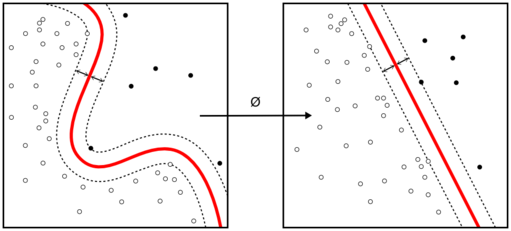
\includegraphics[width=0.8\textwidth]{files/512px-Kernel_Machine.png}
    \caption{Ilustracija kernela za support vector mašinu \cite{SvmImage}}
\end{figure}

Pronalaženje optimalne hiper-ravni se sastoji od minimizovanja $|w|^{2}/2$ u nejednačini $y_j(w*x_j+b) \geq 1$ za svako j. 
Ovo minimizovanje se može uraditi, ako uvedemo Karuš-Kun-Taker množioce (engl. Karush-Kuhn-Tucker multiplier) $\overrightarrow{\alpha} = (\alpha_1,...,\alpha_M)$ i maksimizujemo ih nad Lagranžovoj funkcijom:
\[
    L(\overrightarrow{\alpha}) = \sum_{j=1}^{M}{y_j\alpha_j} - \frac{1}{2}\sum_{j,k=1}^{M}{\alpha_j\alpha_kx_jx_k}
\]
sa sledećim ograničenjima $\sum_{j=1}^{M}{\alpha_j=0}$ i $\forall j \leq M $ $y_j\alpha_j \geq 0$. Tako da, parametri za hiper-ravan se izvode kao:
$w = \sum_{j=1}^{M}\alpha_jx_j$ i $b = y_j - wx_j$ (za one $j$ gde važi da $\alpha_j \neq 0$). Mali broj $\alpha_j$ je različito od nule, takve promenljive se odnose na vektore $x_j$ koji leže na ravni,
ti vektori se zovu \textbf{Potporni vektori}(engl. Support vectors) \cite{rebentrost2014quantum}.

Kernel metoda transformiše podatke u prostor gde su dve klase linearno odvojive. Metoda se oslanja na to da se linearna funkcija
može zapisati isključivo kao skalarni proizvod između primera.
\[
    w^{T}x + b = b + \sum_{i=1}^m \alpha_i x^T x_i
\]
gde je $x_i$ trening primer, a $\alpha$ je vektor koeficijenata. Ovako zapisivanje funkcije nam dozvoljava da zamenimo $x$ sa izlazom funkcije $\phi(x)$, a skalarni proizvod sa funkcijom $k(x,x_i) = \phi(x)*\phi(x_i)$.
Funkcija $k$ se zove \textbf{kernel}, dok funkcija $\phi$ je funkcija koja preslikava podatke iz jednog prostora u drugi. Operator $\langle * \rangle$ predstavlja unutrašnji proizvod ekvivalentno $\phi(x)^T\phi(x_i)$. \cite{goodfellow2016deep}

Kada zamenimo skalarni proizvod sa kernelom, funkciju predikcije možemo da zapišemo kao
\[
    f(x) = b + \sum_i \alpha_{i}k(x,x_i)
\]
Jedna od velikih mana kernel metode jeste da, cena procene izlaza kernel funkcije je linearna u odnosu na broj trening primera, jer $i$-ti indeks označava člana $\alpha_ik(x,x_i)$ kernel funkcije. \cite{goodfellow2016deep} \\
Složenost SVM je $O(log(1/\epsilon)M^2(N+M))$, gde je $\epsilon$ preciznost rešenja, $N$ je broj dimenzija prostora nad kojem radimo, a $M$ je broj trening primera. \\
Takođe krajnje rešenje je binarni klasifikator za neki vektor $x$:
\[
    y(x) = sign(\sum_{j=1}^{M}\alpha_jkk(x,x_j) + b)
\]

\subsubsection{Kvantni algoritam}
Pretpostavimo da imamo metodu za treniranje (engl. Oracle) koja vraća norme $|x_j|$, oznake $y_j$ i kvantne vektore $\Ket{x_j} = \frac{1}{|x_j|}\sum_{k=1}^{N}(x_j)_k\Ket{k}$. \\
Bitno nam je za algoritam da ova metoda vraća podatke pod donjom granicom, da bi se kompleksnost jezgra algoritma mogla iskazati.
Koristeći procenu unutrašnjeg proizvoda za pripremu kernel matrice, može se dobiti SVM algoritam kompleksnosti $O(log(1/\epsilon)M^3 + M^{2}\log(N/\epsilon))$.
Kernel matrica je od velike važnosti za preformulaciju algoritma u vidu funkcije kvadratnog troška. 
Uvodimo pojednostavljanje za nejednakosti, tako što uvodimo promenljivu $e_j$ i koristimo osobinu oznaka da $y_j^2=1$
\[
    y_{j}(w \cdot x_j + b) \geq 1 \to (w \cdot x_j + b) = y_{j} - y_{j}e_{j}
\]
Pored ove jednačine imamo i implicitan uslov Lagranžove funkcije da sadrži kaznenu (engl. penalty) promenljivu
$\gamma/2\sum_{j=1}^{M}e_j^2$, gde je definisan parametar $\gamma$ za relativnu težinu greške treniranja.
Ako uzmemo parcijalni izvod od Lagranžove funkcije i eliminišemo promenljive $u$ i $e_j$ dolazi do aproksimacije funkcije kvadratnog troška problema:
\[
    F\begin{bmatrix}
        b \\
        \overrightarrow{\alpha}
    \end{bmatrix}
    \equiv \begin{bmatrix}
        0 & \overrightarrow{1}^T \\
        \overrightarrow{1} & K+\gamma^{-1} \overrightarrow{1}
    \end{bmatrix}
    \begin{bmatrix}
        b \\
        \overrightarrow{\alpha}
    \end{bmatrix} =
    \begin{bmatrix}
        0 \\
        \overrightarrow{y}
    \end{bmatrix}
\]
Ovde $K_{ij} = x_i^T \cdot x_j$ je simetrična kernel matrica, $y = (y_1,...,y_m)$ kao i
$\overrightarrow{1} = (1,...,1)$. Matrica $F$ je dimenzija $(M+1)\times(M+1)$. Dodatna dimenzija (red i kolona) se sastoji od jedinica,
zbog pomeraja $b$. Promenljiva $\alpha_j$ ima ulogu određivanja distance od optimalnog rešenja. Tako da rešenje, odnosno pronalaženje promenljivih za SVM je oblika:
\[
    \begin{bmatrix}
        b \\
        \overrightarrow{\alpha}
    \end{bmatrix} =
    F^{-1} \begin{bmatrix}
        0 \\
        \overrightarrow{y}
    \end{bmatrix}
\]
U klasičnom algoritmu kompleksnost SVM sa funkcijom kvadratnog troška je $O(M^3)$.

U kvantnom algoritmu, zadatak je generisanje stanja $\Ket{b,\overrightarrow{\alpha}}$ koja opisuju hiper-ravan i onda klasifikuju stanja
$\Ket{x}$. U algoritmu, rešavamo normalizovanu jednačinu $\hat{F}\Ket{b,\overrightarrow{\alpha}} = \Ket{y}$, gde je $\hat{F} = F/trF$ sa 
ograničenjem $\Vert F \Vert \leq 1$. Klasa će biti određenja kao verovatnoća uspeha pri SWAP testu između $\Ket{b,\overrightarrow{\alpha}}$ i
$\Ket{x}$. Za izračunavanje inverzne matrice kvantnim algoritmom, matrica $\hat{F}$ mora da se razdvoji na jednostavne elemente.
Tako da, matrica $\hat{F}$ može da se razdvoji na sledeće elemente $\hat{F} = (J+K+\gamma^{-1}\mathbb{1})/trF$,
gde je matrica
\[
    J = \begin{bmatrix}
        0 & \overrightarrow{1}^T \\
        \overrightarrow{1} & 0 \\
    \end{bmatrix}
\]
Takođe, za procenu faze pravimo formulaciju Lijevog proizvoda \\
$e^{-i\hat{F}\varDelta{t}} = e^{-i\gamma^{-1}\mathbb{1}\varDelta{t}/trF}e^{-iJ\varDelta{t}/trF}e^{-iK\varDelta{t}/trF} + O(\varDelta{t})$.
Za njega važi da ima dve sopstvene vrednosti oblika $\lambda_{\pm} = \pm \sqrt{M}$, a istovetno, 
sopstvena stanja su oblika $\Ket{\lambda_{\pm}} = \frac{1}{\sqrt{2}}(\Ket{0} \pm \frac{1}{\sqrt{M}}\sum_{k=1}^M\Ket{k})$.
Za matricu $\gamma^{-1}\overrightarrow{1}$ dve sopstvene vrednosti su $v_1 = 0$ i $v_2 = \gamma^{-1}M$.
Sada možemo da aproksimiramo fazu za $e^{-i\hat{F}\varDelta{t}}$.

Prvi korak, stanje $\Ket{y}$ može da se transformiše u sopstveno stanje $\Ket{u_j}$ matrice $\hat{F}$, koja ima sopstvenu vrednost $\lambda_j$.
Ono je oblika $\Ket{y} = \sum_{j=1}^{M+1}\braket{u_j|y}\Ket{u_j}$. Ako inicijalizujemo aproksimaciju sopstvene vrednosti na $\Ket{0}$, i primenimo 
procenu faze nad stanjem dobićemo stanje bliže pravoj sopstvenoj vrednosti:
\[
  \Ket{y}\Ket{0} \to \sum_{j=1}^{M+1}\braket{u_j|y}\Ket{u_k}\Ket{\lambda_j} \to \sum_{j=1}^{M+1}\frac{\braket{u_j|y}}{\lambda_j}\Ket{u_j}
\]
Drugi korak, invertujemo dobijeno stanje sopstvene vrednosti, pozivajući rotaciju stanja. Na kraju dobijamo novo stanje sa traženim parametrima SVM ($C = b^2 + \sum_{k=1}^M{\alpha_k}^2$)
\[
    \Ket{b,\overrightarrow{\alpha}} = \frac{1}{\sqrt{C}}(b\Ket{0}+ \sum_{k=1}^M{\alpha_k \Ket{k}})
\]

\paragraph*{Klasifikacija}
Sada imamo trenirani model kvantnog SVM-a i želimo da klasifikujemo stanje $\Ket{x}$. Od stanja $\Ket{b,\overrightarrow{\alpha}}$, korišćenjem metode za treniranje, konstruišemo stanje:
\[
    \Ket{\tilde{u}} = \frac{1}{\sqrt{N_u}}(b\Ket{0}\Ket{0} + \sum_{k=1}^M{\alpha_k |x_k| \Ket{k}\Ket{x_k}})
\]
gde nam je $N_u=b^2+\sum_{k=1}^M{\alpha_k^2 |x_k|^2}$. Pored ovoga konstruišemo i ulazno stanje $\Ket{\tilde{x}}$:
\[
    \Ket{\tilde{x}} = \frac{1}{\sqrt{N_x}}(\Ket{0}\Ket{0} + \sum_{k=1}^M{|x|\Ket{k}\Ket{x}})
\]
gde nam je $N_x=M|x|^2 + 1$. Konstruišemo dva nova stanja $\Ket{\psi}$ i $\Ket{\phi}$; $\Ket{\psi}=\frac{1}{\sqrt{2}}(\Ket{0}\Ket{\tilde{u}}+\Ket{1}\Ket{\tilde{x}})$ i
$\Ket{\phi} = \frac{1}{\sqrt{2}}(\Ket{0}-\Ket{1})$. Merenjem SWAP testa, verovatnoća dobijanja pozitivne vrednosti je $P=|\braket{\psi|\phi}|^2=\frac{1}{2}(1-\braket{\tilde{u}|\tilde{x}})$. 
Ovde dobijamo unutrašnji proizvod, odnosno $\braket{\tilde{u}|\tilde{x}} = \frac{1}{\sqrt{N_xN_u}}(b+\sum_{k=1}^M{\alpha_k |x_k||x|\braket{x_k|x}})$, koji se obično izračunava u $O(1)$ na kvantnom računaru.
Ako hoćemo preciznost $\epsilon$, treba da ponavljamo algoritam merenja $O(P(1-P)/\epsilon^2)$ puta \cite{rebentrost2014quantum}.

\subsection{Kvantna analiza glavnih komponenti}
Ovo je metoda koja se koristi za smanjivanje dimenzija vektora podataka gde nam je bitno da sačuvamo što više informacije o podatku - labava kompresija (engl. lossy compression). 
\subsubsection{Klasičan algoritam}
Neka svaku tačku $x^{(i)} \in \mathbb{C}^n$ želimo da transformišemo u tačku $c^{(i)} \in \mathbb{C}^l$ gde je $l < n$.
Želimo da nađemo funkciju kodiranja koja za ulaz $x$ vraća $c$, odnosno, $f(x)=c$. Takođe želimo da nađemo funkciju dekodiranja $g(f(x)) \approx x$.

Zbog jednostavnosti, uzećemo funkciju množenja matrica kao funkciju dekodiranja. Neka je $g(c)=Dc$, gde je
$D \in \mathbb{C}^{n \times l}$ matrica definisana za dekodiranje. Takođe zbog optimalnog izračunavanja funkcije kodiranja, 
PCA uvodi ograničenje da su kolone međusobno ortogonalne. Još jedno ograničenje koje može da se uvede u algoritam,
koje će dovesti do jedinstvenog rešenja, jeste da su sve kolone matrice $D$ u unitarnoj normi.
Jedan od načina na koji hoćemo da nađemo optimalnu projekciju $c$ za ulaz $x$ jeste da nađemo najmanju $L2$ distancu između ulaza $x$ i dekodovane vrednosti $g(c)$
\[
  c^{*} = \underset{c}{\mathrm{argmin}} \Vert x-g(c) \Vert_2^2.
\]
Ovo pronalaženje minimalne distance će dovesti do optimalnog rešenje problema $c=D^{T}x$ \cite{goodfellow2016deep}. Tako da funkcija enkodovanja je oblika:
\[
f(x) = D^T x
\]
Takođe, možemo da uvedemo novu funkciju rekonstrukcije ulaza $x$
\[
  r(x) = g(f(x)) = DD^T x
\]
Sada treba da se nađe optimalna matrica $D$. Ovo će se rešiti na isti način kao i pronalaženje optimalnog $c$ za ulaz $x$, odnosno kao pronalaženje minimalne $L2$ distance za ulazne vektore
njihove rekonstrukcije
\[
    D^{*} =\underset{D}{\mathrm{argmin}} \sqrt{\sum_{i,j}(x^i_j - r(x^i)_j)^2} \text{ gde važi } D^TD = I_l
\]
Posle procesa izvođenja \cite{goodfellow2016deep}, jednačina za optimalnu matricu $D$ je oblika:
\[
    D^{*} =\underset{D}{\mathrm{argmin}}  Tr(D^TX^TXD) \text{ gde važi } D^TD = I_l
\] 
gde nam je $X \in C^{m \times n}$ matrica gde su redovi ulazni vektori $x$. Ova jednačina se može rešiti koristeći dekompoziciju sopstvenih stanja,
gde bi se pronašli sopstveni vektor za $X^TX$ za najveću sopstvenu vrednost. 
\subsubsection{Kvantni algoritam}
U kvantnom algoritmu bitno nam je da nađemo sopstvene vektore i sopstvene vrednosti za ulaz. Ovo se dosta oslanja na drugi deo metode koji je opisan u sekciji posvećena \textit{Kvantnoj metodi potpornih vektora} .
Ako izaberemo nasumičan vektor $v_j$ iz skupa ulaznih vektora, kreiramo kvantno stanje $\Ket{v_j}$; tada možemo da kreiramo matricu gustine $\rho = (1/N)\sum_j\Ket{v}\Bra{v}$ gde je $N$ veličina skupa vektora. \cite{Quantum_machine_learning}
Slično \textbf{qSVM} nad matricom gustine $\rho$ možemo da apliciramo algoritam procene faze stanja. Odnosno, da primenimo $e^{-i \rho t}$, $t$ puta nad inicijalnim stanjem:
\[
    \Ket{v_j}\Ket{0} \to \sum_i \psi_i\Ket{\chi_i}\Ket{\widetilde{r_i}}
\] 
gde je $\Ket{\chi_i}$ sopstveni vektor od matrice $\rho$, $\widetilde{r_i}$ procena sopstvene vrednosti, a $\psi_i = \Braket{\chi_i|v_j+}$.
I primenom SWAP testa nad dobijenim stanjem, dobijamo stanje:
\[
    \sum_i r_i \Ket{\chi_i}\Bra{\chi_i}\otimes \Ket{\widetilde{r_i}}\Bra{\widetilde{r_i}}
\]
Merenjem ovog stanja mi dobijamo sopstvenu vrednost i sopstveni vektor za matricu gustine $\rho$. Ako uradimo ovaj proces nad većim brojem kopija matrice $\rho$, dobićemo preciznije procene sopstvene vrednosti i sopstvenih vektora. \\
Sada kada imamo sopstvenu vrednost i sopstveni vektor možemo da rekonstruišemo matricu za kodiranje $D$. Vremenska složenost ovog algoritma je $O(\log d)$ \cite{Lloyd_2014}.

\subsection{Kvantna neuralna mreža}
Neuralne mreže su osnova polja koje se naziva \textbf{Duboko učenje} i zato postoji velika pažnja za njihov razvoj.
U radu \cite{Classification_wit_QNN}, autori su predstavili osnove algoritama za Kvantnu neuralnu mrežu (QNN).
U radu su dati neki primeri, neke prednosti i neki nedostaci kvantnog pristupa neuralnim mrežama.

Neka imamo unarni skup stringova $\phi$ oblika $z=z_1 z_2 \dots z_n$ gde svako $z_i$ je bit čija vrednost može da bude $+1$ ili $-1$,
kao i binarne oznake $l(z)$ koje mogu da bude $+1$ ili $-1$. Zbog jednostavnosti neka se u našem skupu nalaze sve permutacije ovako opisanog stringa, to jest neka $|\phi|=2^n$.
Predstavićemo kvantni proces koji radi na $n+1$ kubita (poslednji kubit služi kao izlaz procesa). Kvantni proces se sastoji od unitarnih transformacija ulaznih stanja: ${U_a(\theta)}$.
Svaka transformacija radi nad podskupom ulaznih kubita i zavisi od promenljive $\theta$. Izabraćemo podskup od $L$ transformacija:
\[
  \mathbf{U}(\overrightarrow{\theta}) = U_{L}(\theta_{L}) U_{L-1}(\theta_{L-1}) \dots U_{1}(\theta_{1}) 
\]
koje zavise od $L$ parametara $\overrightarrow{\theta}=\theta_{L} \theta_{L-1} \dots \theta_{1}$. Za svaki string $z$ kreiraćemo početno stanje:
\[
    \Ket{z,1} = \Ket{z_1, z_2, \dots z_n, 1}
\]
Primenjivanje unitarne transformacije vraća stanje: $U(\overrightarrow{\theta})\Ket{z,1}$.
Na izlazu meri se dodati kubit sa Puali-jevim operatorom $\sigma_y$, koji se kasnije naziva i $Y_{n+1}$.
Tako da na kraju imamo izlaz $+1$ ili $-1$. Cilj je isti kao i kod klasičnih neuralnih mreža, a to je da se nauči proces da vraća tačne vrednosti za dati ulazni string.
Pošto merenje izlaznog kubita nije sigurno, odnosno merenjem kubita dobijamo tačnu vrednost sa nekom verovatnoćom, uvodimo transformaciju:
\[
    \bra{z,1}U^T(\overrightarrow{\theta})Y_{n+1}U(\overrightarrow{\theta})\Ket{z,1}
\]
koja predstavlja prosečnu vrednost merenja, ako $Y_{n+1}$ merimo na više kopija originalnog izlaza.

Ovde, kao i u klasičnoj neuralnoj mreži, cilj nam je da nađemo parametar $\overrightarrow{\theta}$ koja vraća tačnu vrednost sa velikom preciznošću.
Slično prethodnoj postavci imamo: $L$ unitarnih promenljivih sa korespondentnim promenljivama $\overrightarrow{\theta}$, kao i ulazni string $z$; 
tada možemo da predstavimo funkciju troška kao:
\[
    \mathit{loss}(\overrightarrow{\theta},z) = 1 - l(z)\bra{z,1}U^T(\overrightarrow{\theta})Y_{n+1}U(\overrightarrow{\theta})\Ket{z,1}
\]
Možemo primetiti da ova funkcija troška je linearna i da je minimum u $0$, jer je vraćena vrednost između $-1$ i $+1$.
Pretpostavimo da kvantna neuralna mreža radi savršeno, tako da za svaki ulazni string $z$, merenje uvek vraća tačnu oznaku.
To onda znači da optimalna promenljiva $\overrightarrow{\theta}$ postoji i da je minimum za funkciju troška u $0$ za sve ulaze $z$.

Neka imamo skup stringova \(S\) za treniranje, sa njihovim oznakama. Postoji kvantni proces koji ima mogućnost da
prikaže tražene oznake i zavisi od parametara $\overrightarrow{\theta}$. Opisaćemo proces kako da dođemo do optimalnih parametara $\overrightarrow{\theta}$.
Neka počnemo sa nasumičnom promenljivom $\overrightarrow{\theta}$ (ili ako imamo neku pretpostavku početne vrednosti parametara). Izaberimo neki string $z^1$ iz skupa za treniranje.
Primenjujemo kvantni proces nad izabranim stringom:
\[
    U(\overrightarrow{\theta})\Ket{z,1}
\] 
i merimo $Y_{n+1}$ na zadnjem kubitu. Nakon nekoliko merenja možemo da imamo dobru aproksimaciju očekivane vrednosti od $Y_{n+1}$
i tada izračunavamo $\mathit{loss}(\overrightarrow{\theta},z^1)$. Nakon toga, želimo da promenimo parametar $\overrightarrow{\theta}$ tako da smanjimo
funkciju troška za string $z^1$. Postoje dva načina da se uradi traženo: (1) da uradimo pomeraj ka nekom izabranom uzorku u $[\overrightarrow{\theta}-\epsilon,\overrightarrow{\theta}+\epsilon]$ intervalu,
(2) da izračunamo izvod funkcije troška po $\overrightarrow{\theta}$ i da se malo pomerimo ka pravcu koji minimizuje funkciju.
Ovo nam daje novi parametar $\overrightarrow{\theta^1}$. Sada biramo ponovo iz skupa neki string $z^2$ i ponavljamo prethodni proces ali sa parametrom $\overrightarrow{\theta^1}$.
Ovako dobijamo novi parametar $\overrightarrow{\theta^2}$ koji ima manju funkciju troška za string $z^2$ nego parametar $\overrightarrow{\theta^1}$.
Ovako prolazimo kroz proces sve dok ne prođemo kroz ceo skup $S$. Kao rezultat ovoga generisana je sekvenca parametara $\overrightarrow{\theta^1}, \overrightarrow{\theta^2}, \dots \overrightarrow{\theta^S}$.
Ako je učenje parametara uspešno, onda bi bilo dobijeno da operator $U(\overrightarrow{\theta^S})$, kada se primeni na stanju $\Ket{z,1}$, vraća stanje koje kada se izmeri na izlazu vraća tačnu oznaku $l(z)$.
Ako je $z$ iz skupa za treniranje, reći ćemo da je model naučio podatke za treniranje. Ako je $z$ izvan skupa za treniranje, možemo reći da je model naučio da generalizuje i za neviđene podatke.

Ovaj proces koji je opisan, može se primetiti, u klasičnom mašinskom učenju zove se \textit{stohastičko učenje}.
U tradicionalnom mašinskom učenju sa neuralnim mrežama, parametri se prikazuju kao promenljive unutar matrice, koja je linearna u odnosu na unutrašnje vektore.
Nad komponentama tih vektora vrše se nelinearne transformacije, pre nego što se pomnože sa ostalim parametrima. 
Uvođenje dobre nelinearnosti je jedan od glavnih delova uspešne implementacije modela u klasičnom mašinskom učenju.
Ovu osobinu klasičnih neuralnih mreža teško je prebaciti u kvantni sistem, jer je kvantna mehanika, osnova celog koncepta kvantnog računarstva, sama po sebi linearna.
U metodi koja je opisana, svaka unitarna operacija se izvršava nad izlazom prethodne operacije, pri čemu se između operacija ne izvršava nikakva nelinearna transformacija.
Neka nam je svaka unitarna transformacija oblika $e^{i\theta\Sigma}$, gde je $\Sigma$ proizvod tenzora koji se sastoji iz skupa Pauli-jevih operatora, koji rade nad nekolicinom kubita.
Izvod operatora po $\overrightarrow{\theta}$ je ograničen po $L$, to jest po broju parametara. Ovo je značajno, jer znači da gradijent ne može da ode u beskonačnost i tako izbegavamo 
veliki problem koji se može desiti klasičnim neuralnim mrežama.

\begin{figure}[ht]
    \centering
    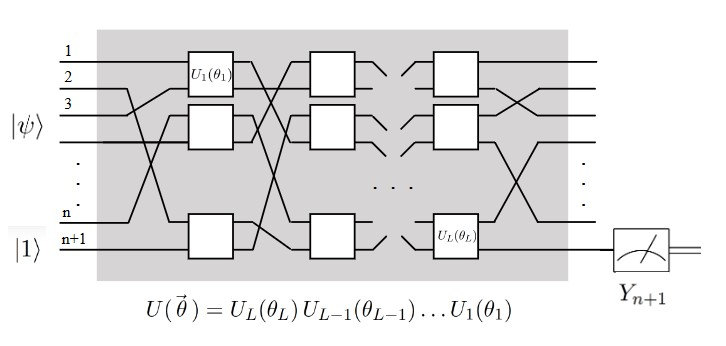
\includegraphics[width=0.9\textwidth]{files/QNN.jpg}
    \caption{Ilustracija kvantne neuralne mreže \cite{Classification_wit_QNN}}
\end{figure}

\subsubsection{Reprezentacija modela}
Neka imamo $2^n$, $n$-bitnih stringova i vezano za njih $2^{(2^n)}$ funkcija oznaka $l(z)$.
Ako nam je data određena funkcija oznaka, onda možemo da definišemo operator nad baznim stanjima kao:
\[
    U_l\Ket{z,z_{n+1}} = e^{i\frac{\pi}{4}l(z)X_{n+1}}\Ket{z,z_{n+1}}
\]
Ovaj operator rotira ulazni kubit oko $x$-ose za $\frac{\pi}{4}$ puta oznaka za string $z$.
Tako da iz toga imamo:
\[
    U_l^TY_{n+1}U_l = \cos(\frac{\pi}{4}l(Z))Y_{n+1} + sin(\frac{\pi}{4}l(Z))Z_{n+1}
\]
gde u formuli, $l(Z)$ je interpretirana kao operator dijagonalan u odnosu na bazna stanja.
Takođe, pošto funkcija oznaka l(z) može da vrati ili $+1$ ili $-1$, iz toga imamo $\bra{z,1}U_l^TY_{n+1}U_l\ket{z,1} = l(z)$.
Ovo nam pokazuje da bar na nekom apstraktnom nivou imamo mogućnost da predstavimo bilo koju funkciju oznake kao kvantno kolo.

Sada ćemo objasniti kako da se napiše operator $U_l$ kao proizvod dve kubit unitarne transformacije. Zbog ovoga, treba da se pređe na \textit{boolean} promenljive $b_i=\frac{1}{2}(1-z_i)$ i 
neka funkcija oznake $l$ bude oblika $1-2b$ gde je $b \in \{0,1\}$. Sada možemo da iskoristimo \textbf{Reed-Muller} zapisivanje bilo koje \textit{boolean} funkcije u obliku bitova $b_1 \dots b_n$:
\[
    b = a_0 \oplus (a_1b_1 \oplus a_2b_2 \oplus \dots a_n b_n) \oplus (a_{12}b_1b_2 \oplus a_{13}b_1b_3 \oplus \dots) \oplus \dots \oplus a_{12 \dots n}b_1b_2 \dots b_n
\]
gde su koeficijenti $a \in \{0,1\}$. Primećuje se da imamo $2^n$ koeficijenta, pošto su oni ili 0 ili 1, da stvarno ima $2^{(2^n)}$ mogućih \textit{boolean} funkcija.
Naša funkcija $b$ može biti eksponencijalno dugačka. Sada možemo da zapišemo unitarnu transformaciju koja zavisi od funkcije oznaka kao:
\[
    U_l = e^{i\frac{\pi}{4}X_{n+1}}e^{-1\frac{\pi}{2}BX_{n+1}}
\]
gde je $B$ operator, dijagonalan u odnosu na bazna stanja, koji odgovara datoj funkciji $b$. 
Svaka vrednosti u $B$ se množi sa $X_{n+1}$ tako da svaka vrednost je komutativna sa ostalim vrednostima. 
Svaki član, različit od nule, u \textbf{Reed-Muller} formuli dovodi do kontrolnog \textit{bit-flip}-a u $U_l$ na izlaznom kubitu.

Ovaj rezultat kvantnog predstavljanja ima analog u klasičnoj teoriji predstavljanja \cite{Cybenko1989ApproximationBS}.
Ona pokazuje da bilo koja \textit{boolean} funkcija oznake može da se predstavi u neuralnoj mreži dubine tri, gde srednji slog ima veličinu $2^n$.
Ovako velika matrica ne bi mogla da se predstavi na klasičnim računarima, ali bi mogli na kvantnim računarima, koji po prirodi rade
nad Hilbertovim prostorima sa eksponencijalnim dimenzijama. Ali još nije dokazano da svaka \textit{boolean} funkcija može da se predstavi u kvantnom kolu koje nije eksponencijalne dubine.

\paragraph*{Reprezentacija parnosti podskupa}
Neka imamo datu funkciju oznaka koja vraća parnost podskupa bitova datog stringa. Neka je podskup $\mathbb{S}$
i neka je $a_j=1$ ako je bit $j$ u podskupu i $a_j=0$ ako $j$ nije u podskupu. Reed-Muller formula za parnost podskupa je:
\[
    P_{\mathbb{S}}(z) = \sum_j \oplus a_j b_j
\]
Ovo nam dozvoljava da napravimo unitarnu transformaciju koja implementira parnost podskupa:
\[
    U_{P_{\mathbb{S}}} = e^{i\frac{\pi}{4}X_{n+1}}e^{-i\frac{\pi}{2}\sum_j a_jB_jX_{n+1}}
\]
Kolo se sastoji od, najviše, $n$ operatora nad dva kubita koji su međusobno komutativni, gde je pridodati kubit u svim operatorima nad dva kubita.

\subsubsection{Učenje modela}
U ovoj podsekciji će biti objašnjene dve potencijalne metode kako da se menja parametar $\overrightarrow{\theta}$ tako da se funkcija troška smanjuje.
Ako su nam dati parametri $\overrightarrow{\theta}$ i trening primer $z$, prvo procenjujemo vrednost troška od $\mathit{loss}(\overrightarrow{\theta},z)$.
Da bismo ovo uradili treba da napravimo više merenja $Y_{n+1}$ za $U(\overrightarrow{\theta})\Ket{z,1}$.
Da bismo ovo uspeli sa verovatnoćom većom od $99\%$ za procenu od funkcije troška koja je u $\delta$ intervalu od prave vrednosti funkcije troška
treba da napravimo najmanje $2/\delta^2$ merenja ($\delta \in (0,1)$).

Nakon što procenimo vrednost funkcije troška želimo da izračunamo gradijent funkcije troška u odnosu na $\overrightarrow{\theta}$.
Jedan od načina jeste da menjamo jednu po jednu promenljivu u $\overrightarrow{\theta}$. Nakon svake promene treba da se izračuna
$\mathit{loss}(\overrightarrow{\theta'},z)$, gde $\overrightarrow{\theta'}$ je različit od $\overrightarrow{\theta}$ za neku malu vrednost u jednoj promenljivoj.
Ako bi se koristio simetričan izvod funkcije troška svaku promenljivu parametra bismo mogli da izračunamo do preciznosti $\eta$ u oko $1/\eta^3$ merenja.
Ovaj proces bi trebalo da se ponavlja $L$ puta da bi se dobio puni gradijent.

Alternativna strategija jeste da se menja svaka promenljiva gradijenta, što se koristi kada su sve unitarne transformacije oblika $e^{i\theta\Sigma}$.
Ako posmatramo izvod za funkciju troška $\mathit{loss}(\overrightarrow{\theta},z)$ za parametar $\theta_k$, koji je vezan za transformaciju $U_k(\theta_k)$
(koja ima i generalni Pauli-jev operator $\Sigma_k$). Sada:
\[
    \frac{d\mathit{loss}(\overrightarrow{\theta},z)}{d\theta_k} = 2Im(\Bra{z,1}U_1^T \dots U_L^TY_{n+1}U_L \dots U_{k+1} \Sigma_k U_k \dots U_1 \Ket{z,1})
\]
Ako primetimo da su $Y_{n+1}$ i $\Sigma_k$ unitarni operatori, tada definišemo unitarni operator:
\[
    \mathcal{U}(\overrightarrow{\theta}) = U_1^T \dots U_L^TY_{n+1}U_L \dots U_{k+1} \Sigma_k U_k \dots U_1
\]
tako da izvod možemo da zapišemo kao:
\[
    \frac{d\mathit{loss}(\overrightarrow{\theta},z)}{d\theta_k} = 2Im(\Bra{z,1}\mathcal{U}\Ket{z,1})
\]
$\mathcal{U}(\overrightarrow{\theta})$ se može posmatrati kao kvantno kolo koje sadrži $2L+2$ unitarnih transformacija.
Sada možemo da primenimo $\mathcal{U}(\overrightarrow{\theta})$ nad stanjem $\Ket{z,1}$. Ako koristimo dodati kubit, možemo da merimo imaginarni deo
izvoda funkcije. Započećemo sa stanjem $\Ket{z,1}\frac{1}{\sqrt{2}}(\Ket{0}+\Ket{1})$ i primenićemo $i\mathcal{U}(\overrightarrow{\theta})$ nad dodatim kubitom vrednosti $1$.
Ovo kreira:
\[
    \frac{1}{\sqrt{2}}(\Ket{z,1}\Ket{0} + i\mathcal{U}(\overrightarrow{\theta})\Ket{z,1}\Ket{1})
\]
Ako primenimo Hademardovu kapiju na dodatim kubitom dobijamo:
\[
    \frac{1}{2}(\Ket{z,1}+\mathcal{U}(\overrightarrow{\theta})\Ket{z,1}\Ket{0}) + \frac{1}{2}(\Ket{z,1}-i\mathcal{U}(\overrightarrow{\theta})\Ket{z,1}\Ket{1})
\]
Sada kada izmerimo dodati kubit, verovatnoća da se dobije $0$ je:
\[
    \frac{1}{2} - \frac{1}{2}Im(\bra{z,1}\mathcal{U}(\overrightarrow{\theta})\Ket{z,1})
\]
tako da, ponavljanjem ovog merenja možemo da dobijemo dobru procenu imaginarnog dela stanja iz kojeg možemo da izvučemo procenu $k$-te komponente traženog gradijenta.
Ovaj metod izbegava numeričke nepreciznosti prethodne strategije. Cena ove metode je potreba za dodatnim kubitom kao i za kvantnim kolom $2L+2$ dubine.

Pošto smo izračunali gradijent, treba nam metod za izmenu $\overrightarrow{\theta}$. Neka je $\overrightarrow{g}$ gradijent funkcije troška po parametru $\overrightarrow{\theta}$.
Sada menjamo $\overrightarrow{\theta}$ u pravcu $\overrightarrow{g}$. Sa veličinom koraka $\gamma$ imamo
\[
    \mathit{loss}(\overrightarrow{\theta}+\gamma \overrightarrow{g}) = \mathit{loss}(\overrightarrow{\theta},z)+ \gamma \overrightarrow{g}^2 + O(\gamma^2)
\]
Pošto želimo da smanjimo trošak na $0$ možemo da napravimo da:
\[
    \gamma = -\frac{\mathit{loss}(\overrightarrow{\theta},z)}{\overrightarrow{g}^2}
\]
Ovako nešto bi dovelo da trošak bude $0$ za trenutni primer, ali može da dovede do loših efekata za ostale primere.
Ovde se u klasičnom mašinskom učenju obično uvodi promenljiva, stepen učenja $r \in (0,1]$ i onda imamo sledeće:
\[
    \overrightarrow{\theta} \to \overrightarrow{\theta} - r(\frac{\mathit{loss}(\overrightarrow{\theta},z)}{\overrightarrow{g}^2})\overrightarrow{g}
\]
Deo uspešne implementacije mašinskog učenja je da racionalno odaberemo vrednost stepena učenja.

\paragraph{Učenje parnosti podskupa}
Za dati podskup $\mathbb{S}$, unitarna transformacija $U_{P_\mathbb{S}}$ može da prikaže parnost podskupa za sve ulazne stringove.
Da bi se naučio skup unitarnih operacija koje zavise od parametara, sa tim da za svaki podskup postoje parametri koji opisuju $U_{P_\mathbb{S}}$,
najlakši način da se ovo postigne jeste da se koriste $n$ parametara
\[
    U(\overrightarrow{\theta}) = e^{i\frac{\pi}{4}X_{n+1}}e^{-i\sum_j^n \theta_jB_jX_{n+1}}
\]
Ovde se vidi da je reprezentacija savršena kada je $\theta_j = \frac{\pi}{2}$ ako je $j$ u podskupu i $\theta_j = 0$ ako $j$ nije u podskupu.
Posle eksperimenta sa malim brojem kubita gde su uspeli da nauče model, njihov argument je da sa povećanjem veličine sistema postaje nemoguće da se nauči kvantni model.
Da bi to pokazali, izračunali eksplicitnu formulu za očekivanu vrednost za $Y_{n+1}$
\[
    \bra{z,1}U^T(\overrightarrow{\theta})Y_{n+1}U(\overrightarrow{\theta})\Ket{z,1} = \cos(2\sum_j\theta_jb_j)
\]
Sa oznakom $l(z)$, ovo može se ubaciti u funkciju troška, ali sada može da se izračuna prosek
troška za sve $2^n$ stringove, jer imamo eksplicitnu formulu za oznake i njihovo očekivanje.
Postoji više verzija izračunate funkcije, koja zavisi od izlaza $n \bmod 4$ i koliko bitova se nalazi u podskupu $\mathbb{S}$.
Za prikaz uzeli su primer gde je $n$ deljiv sa 4 i skup $\mathbb{S}$ sadrži svih $n$ bitova.
U tom slučaju prosečan trošak za sve stringove je 
\[
    1 - \cos(\theta_1 + \theta_2 + \dots \theta_n)sin(\theta_1)sin(\theta_2) \dots sin(\theta_n)
\]
Iz formule se vidi da je u minimumu kada su sve $\theta=\frac{\pi}{2}$. Zamislite kakva bi bila pretraga minimuma (pored ovog primera) funkcije
nad intervalom $[0\;\pi]^n$. Funkcija bi samo prikazivala vrednosti eksponencijalno blizu $1$, sem u eksponencijalno malim intervalima oko optimalnih uglova.
Isto tako gradijent bi bio veoma mali sem oko optimalnih uglova. Zato čak i ako imamo pristup prosečnom trošku, nijedan metod koji se oslanja na gradijentni pristup
ne bi mogao biti korišćen za pronalaženje optimalnog ugla za bilo koji primer sa povećim $n$, gradijent bi radio izvan preciznosti mašine u tom slučaju.

\subsubsection{Učenje osobina kvantnih stanja}
Sa kvantnom neuralnom mrežom, očekuje sa da na ulazu može da ima bilo koje kvantno stanje (koje nije izvedeno iz nekog klasičnog podatka)
i da može da nauči neke njegove osobine i da ih izbaci u obliku nekih oznaka. Ne postoji ni jedna klasična neuralna mreža koja može to da uradi, jer klasični računari ne mogu da prihvate kvantno stanje kao ulaz.
Osnovna ideja je da se $n$-kubitno stanje $\Ket{\psi}$ ubaci u kvantnu neuralnu mrežu sa dodatim kubitom, koji služi za čitanje rezultata, koji je postavljen na $1$.
Neka nam je data unitarna transformacija $U(\overrightarrow{\theta})$ tako da imamo stanje
\[
    U(\overrightarrow{\theta})\Ket{\psi,1}
\] 
i onda merimo $Y_{n+1}$. Cilj ovoga je da namestimo da izlaz ovog merenje bude ekvivalentan nekim dvema oznakama koje označavaju neke osobine kvantnog stanja.
To je prikazano u sledećem primeru.
Posmatrajmo Hamiltonov operator $H$ (engl. Hamiltonian), koji je suma lokalnih vrednosti sa dodatnom osobino da ima i pozitivne i negativne sopstvene vrednosti.
Sa datim kvantnim stanjem $\ket{\psi}$, obeležava se oznakom koja pokazuje da li je očekivana vrednost Hamiltonovog operatora pozitivna ili negativna:
\[
    l(\Ket{\psi}) = sign(\bra{\psi}H\Ket{\psi})
\]
Posmatrajmo operator $U_H(\beta) = e^{i\beta HX_{n+1}}$, gde je $\beta$ mala i pozitivna vrednost. Sada
\[
    \Bra{\psi,1}U_H^T(\beta)Y_{n+1}U_H(\beta)\Ket{\psi,1} = \bra{\psi}sin(2\beta H)\Ket{\psi}
\]
tako da za dovoljno malo $\beta$ ovo je približno jednako $2\beta\bra{\psi}H\Ket{\psi}$ i tako imamo znak očekivane vrednosti za 
predikciju oznake, koja je jednaka tačnoj oznaci. Ovako prikazana, ovo je funkcija oznake sa kvantnim kolima koja ima malu grešku.
Mala greška dolazi iz toga što je $\bra{\psi}sin(2\beta H)\Ket{\psi}$ samo približno jednako $2\beta\bra{\psi}H\Ket{\psi}$
Ako uzmemo da $\beta$ bude dosta manje od $1/\Vert H \Vert$ (inverzno od norme matrice $H$), možemo da napravimo da nam greška bude mala.

Posmatrajmo graf gde na svakoj ivici imamo \textit{ZZ} uparivanje sa koeficijentom ili $+1$ ili $-1$.
Hamiltonov operator je oblika: $H = \sum_{i,j}J_{ij}Z_iZ_j$ gde prvobitna suma je ograničena na ivice grafa i $J_{ij}$ je ili $+1$ ili $-1$.
Neka postoje $M$ vrednosti u $H$. Prvo, treba da izaberemo $M$ uglova $\theta_{ij}$ i neka je kvantno kolo koje implementira transformaciju oblika:
\[
    U(\overrightarrow{\theta}) = e^{i\sum_{i,j}J_{ij}Z_iZ_jX_{n+1}}
\]
Ako izaberemo $\theta_{ij}=\beta J_{ij}$ imamo operator $U_H(\beta)$ koji osigurava da možemo da označimo traženu oznaku ako izaberemo malo $\beta$.\\
Kvantno stanje $\Ket{\psi}$ je u Hilbertovom prostoru sa $2^n$ dimenzija i ne možemo da očekujemo da naučimo oznake za svako stanje.
Posmatrani Hamiltonov operator ima bitovsku strukturu, tako da možemo da se ograničimo kvantna stanja sa bitskim strukturama.
Tako je predloženo da se za treniranje koriste stanja samo sa ovom formom, kao i za testiranje.
\newpage
\section{Zaključak}
U ovom radu je prikazano kraći uvod u kvantno računarstvo i kvantno mašinsko učenje. Takođe je dato nekoliko primera metoda kvantnog mašinskog učenja, 
koji poboljšavaju svoje klasične ekvivalente. Glavni izazov trenutno je praktična primena, koja je strogo vezana za razvoj funkcionalnih kvantnih računara.

Ostavljeno je dosta metoda kvantnog mašinskog učenja, koje čitalac može da istraži, ali su ove prikazane verovatno dovoljne za razumevanje oblasti.
Trenutak kada se dokaže kvantna nadmoć dovešće do većeg zainteresovanja ka svim oblastima povezane za kvantno računarstvo, 
uključujući i kvantno mašinsko učenje. Svakako se savetuje praćenje daljeg razvoja ove oblasti, pošto je ona relativno mlada
i ima dosta inovacija i poboljšavanja.


\newpage

\printbibliography

\end{document}